\section{Characterization method and results}
\label{Method}
% The setup of the experiment and preanalysis are discussed in sec.~\ref{sec:laserstage}. Analysis method and results of parameters are introduced in the following sections.
\subsection{Setup and preanalysis}
\label{sec:laserstage}

To obtain single PE events, the laser intensity is adjusted to the level of $\frac{1}{20}$ occupancy. The window size $T_{\mathrm{wave}}$ is \SI{10400}{ns} to include all the possible after-pulses (sec.~\ref{sec:afterpulse}). The rising edge of trigger waveform from the laser system is linearly interpolated to get the half-height time $t_{\mathrm{trig}}$ at about \SI{200}{ns} as shown in Fig.~\ref{fig:triggertime}.
\begin{figure}[!htbp]
    \centering
    \includegraphics[width=\LF\textwidth]{figures/method/triggerwave.pdf}
    \caption{An example of waveform and trigger signals. The orange line is the trigger waveform, with its high and low voltages indicated by two black horizontal dashed lines. The green cross is the interpolated trigger time. The blue solid line shows the PMT waveform with a PE pulse. The horizontal violet dotted line is the voltage threshold for calculating the baseline shown by the blue horizontal dashed line. Linearly interpolated 10\% and 90\% of (downward) rising and falling edges are represented by the green and cyan rectangles. Red and yellow vertical dash lines respectively are the 10\% rising edge and the pulse peak.}
    \label{fig:triggertime}
\end{figure}

To accelerate calculation, the maximum pulse is searched in a preanalysis window $[t_{\mathrm{trig}},600\,\mathrm{ns}]$. The number of dark noise in each waveform obeys Poisson distribution with expectation being about 0.008 for \SI{20}{kHz} DCR, while the expected number of laser pulse is about 0.05, which dominate the dataset. The peak time $t_p$ is the position of minimum in each waveform as shown in Fig.~\ref{fig:triggertime}.
%Because the maximum pulse is selected in each waveform, the expected charge distribution is the distribution of $\max(C_n)$ ($n=1,...,N$), in which $C_n$ is the charge of the nth PE and $N$ is the number of PE in a waveform.
Besides, the charge bias caused by the small ratio multi-PE cases is omitted.

Due to the baseline being not zero, a set of baseline intervals is selected using a voltage threshold, as horizontal violet dotted line shown in Fig.~\ref{fig:triggertime}, to remove potential pulses from the time window $[-200\,\mathrm{ns},-10\,\mathrm{ns}]$ and $[100\,\mathrm{ns},200\,\mathrm{ns}]$ relative to $t_p$. The selected areas are cut off \SI{10}{ns} at both ends to remove the rising edge and falling edge of potential pulses. The baseline $\mu_b$ and fluctuation $\sigma_b$ are estimated as average and the standard deviation of the rest waveform. The peak height $V_p$ of a pulse is the difference between $\mu_b$ and minimum of the pulse.

To reduce the impact of dark noise, a gaussian function G$(\mu_{t0},\sigma_{t0})$ is unbinned fitted to the distribution of $t_p-t_{\mathrm{trig}}$ of pulses whose $V_p$ exceeds \SI{5}{ADC} in preanalysis and all the characterizations include $t_p$ and $V_p$ are calculated in a shorter candidate window $[\mu_{t0}-5\sigma_{t0}, \mu_{t0}+5\sigma_{t0}]$.

\subsection{Peak and charge spectrum}
\label{sec:noisepeak}

Considering the rise time and fall time distribution, the equivalent charge $C_{\mathrm{equ}}$ of a pulse is calculated as summation of the amplitudes without baseline in a time window $[-10, 75]$\,ns relative to $t_p$ of the signal as illustrated in the pink region in Fig.~\ref{fig:triggertime}, with an integration window $T_s=85\,\mathrm{ns}$. Due to the input impedance being \SI{50}{\Omega} \cite{CAENV1751}, the true charge $C$ of the pulse is $\frac{C_{\mathrm{equ}}}{50 \Omega}$.

Fig.~\ref{fig:triggercharge} shows the distribution of $C_{\mathrm{equ}}$ of an MCP-PMT. The pedestal is a set of waveforms with no signal, of which $C_{\mathrm{equ}}$ is the summation of fluctuation and obeys Gaussian distribution $G(0, T_s\sigma_b^2)$, in which $\sigma_b$ is the standard deviation of the white noise of baseline mentioned in sec.\ref{sec:laserstage}. The  main peak $C_1$ in $C_{\mathrm{equ}}$ distribution is fitted in sec.\ref{sec:noisegain}. To remove the influence of the pedestal and describe the long tail in the charge distribution, pulses of which $V_p$ higher than \SI{3}{ADC} and $C_{\mathrm{equ}}$ larger than 0.25$C_1$ are selected to calculate mean $\mu_{C}$ and sample variance $s^2_{C}$ of $C_{\mathrm{equ}}$. Due to the influence of long tail, $\mu_{C}$ is larger than $C_1$. The long tail has been referred to in \cite{JUNOMassTesting} and parameterized in \cite{JUNOLongtail} but without dedicated consideration of the multiplication process of the photoelectron. The physical model and solution of the long tail in charge distribution will be discussed in our future work. The $V_p$ distribution with \SI{1}{ADC} bin width in Fig.~\ref{fig:triggerpeak} illustrates \SI{3}{ADC} and 0.25$C_1$ threshold are complementary to exclude some noise with small $V_p$ but large $C_{\mathrm{equ}}$.

\begin{figure}[!htbp]
    \centering
    \begin{subfigure}[b]{\SF\textwidth}
        \includegraphics[width=\textwidth]{figures/method/triggercharge.pdf}
        \caption{}%PM
        \label{fig:triggercharge}
    \end{subfigure}
    \begin{subfigure}[b]{\SF\textwidth}
        \includegraphics[width=\textwidth]{figures/method/triggerpeak.pdf}
        \caption{}%PM
        \label{fig:triggerpeak}
    \end{subfigure}
    \caption{(a) Charge distribution of an example MCP-PMT. The vetical blue dash line is the cut for charge. The orange histogram is the selected waveforms with peak cut. The pink area and green area are respectively the fit interval for the peak and vally of charge distribution. (b) Peak distribution of an example MCP-PMT. The vertical green dash line is the cut for the peak. The orange histogram is the selected waveforms with charge cut.}
\end{figure}

\subsection{Gain and single PE resolution}
\label{sec:noisegain}

There exists a long tail in the charge distribution as shown in the histogram in Fig.~\ref{fig:triggercharge}. To describe the energy resolution of the main peak of the charge distribution, a gaussian function G$(C_1,\sigma^2_{C_1})$ is used to fit the binned data in an interval $[0.65C_1, 1.35C_1]$ via the modified least-square (MLS) method \cite{Cowan1998StatisticalDA} as the red line shown in Fig.~\ref{fig:triggercharge}. The gain of the main peak $G_1$ and the gain of the total charge $G$ of single PE are respectively calculated as $\frac{C_1}{e\times 50\Omega}$ and $G\frac{\mu_{C}}{e\times 50\Omega}$, in which $e$ is the charge of an electron. The main peak resolution $\mathrm{Res}_1$ and the total charge resolution $\mathrm{Res}$ are defined as $\frac{\sigma_{C_1}}{C_1}$ and $\frac{\sqrt{s^2_{C}}}{\mu_{C}}$.

Fig.~\ref{fig:totalchargeCompare} shows the 2d distribution of the gain and resolution. $G$ is about 2 times $G_1$ for the MCP-PMTs. Although mean of $\mathrm{Res}_1$ of MCP-PMTs is about 0.25, the long tail leads that mean of $\mathrm{Res}$ is about 0.69, worse than the reference PMT.

\begin{figure}[!htbp]
    \centering
    \includegraphics[width=\MF\textwidth]{figures/result/gainres.pdf}
    \caption{The gain and resolution of main peak and total charge. Geen points represent the reference PMT and red points represent MCP-PMTs. Cross markers represent $G_1$ and $\mathrm{Res}_1$. Plus markers represent $G$ and $\mathrm{Res}$.}
    \label{fig:totalchargeCompare}
\end{figure}

\subsection{Peak-to-valley (P/V) ratio}
A parabolic function is fitted to the valley based on the MLS method in the interval $[-0.15C_1, 0.25C_1]$ relative to the least count bin of histogram between pedestal and single PE peak as shown in Fig.~\ref{fig:triggercharge}. The local minimum $N_v$ of the charge spectrum is calculated as the minima of the parabolic function. The $N_p$ is the peak of the Gaussian function described in sec.~\ref{sec:noisegain}. The P/V ratio is $\frac{N_p}{N_v}$ and shows the ability to discriminate between electronic noise and true signal. The mean P/V ratio of MCP-PMTs is about 5.8 while that of the reference PMT is about 2.4.

\subsection{Rise time, fall time, and full width at half maximum (FWHM)}
As shown in Fig.~\ref{fig:triggertime}, $t^{10}_r$, $t^{50}_r$, $t^{90}_r$ are the time of 10\%, 50\%, and 90\% $V_p$ in the rising edge and $t^{10}_f$, $t^{50}_f$, $t^{90}_f$ are the time of 10\%, 50\%, and 90\% $V_p$ in the falling edge which are acquired via linear interpolation method. The rise time, fall time, and FWHM are calculated as follows: $t_r = t^{90}_r - t^{10}_r$, $t_f = t^{10}_f - t^{90}_f$, $\mathrm{FWHM} = t^{50}_f - t^{50}_r$. Estimated mean and deviation of rise time, fall time, and FWHM are $3.71\pm0.15$\,ns, $15.6\pm1.8$\,ns, and $9.07\pm0.63$\,ns for 9 MCP-PMTs.

\subsection{Transit time spread (TTS)}
The photoelectrons generated from the cathode drift to the MCP in the electric field as shown in Fig.~\ref{fig:mcpelectron}. The drift time is determined by the initial kinetic of photoelectrons and the electric field. A simple model consisting of a cathode, a focusing electrode, and an MCP with \SI{0}{V}, \SI{480}{V}, and \SI{528}{V} is constructed to simulate the electric field and the electron trajectory. The drift times of the electrons at the top of PMT with \SI{0}{eV} and \SI{3}{eV} are respectively about \SI{21}{ns} and \SI{18}{ns}. The electrons hitting the channels of MCP are multiplied and generate observable signals, while the electrons hitting on the surface of MCP generate the secondary electrons (including a single elastic scattering electron), which drift in the electric field until hitting on the MCP again and generate delayed pulses \cite{KM3NetTesting}. Multiple secondary electrons with different kinetic energy may cause two or more pulses due to different drift time of secondary electrons as shown in Fig.~\ref{fig:triggerTT2pulse}.

\begin{figure}[!htbp]
    \centering
    \begin{subfigure}[t]{\SF\textwidth}
        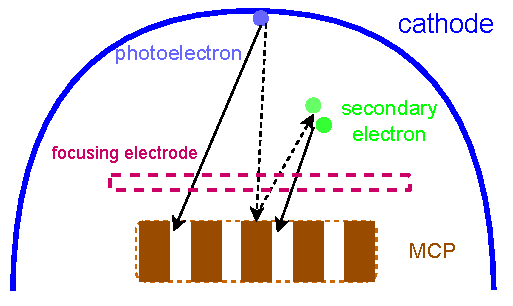
\includegraphics[width=\textwidth]{figures/method/MCPelectron.pdf}
        \caption{}%PM
        \label{fig:mcpelectron}
    \end{subfigure}
    \begin{subfigure}[t]{\SF\textwidth}
        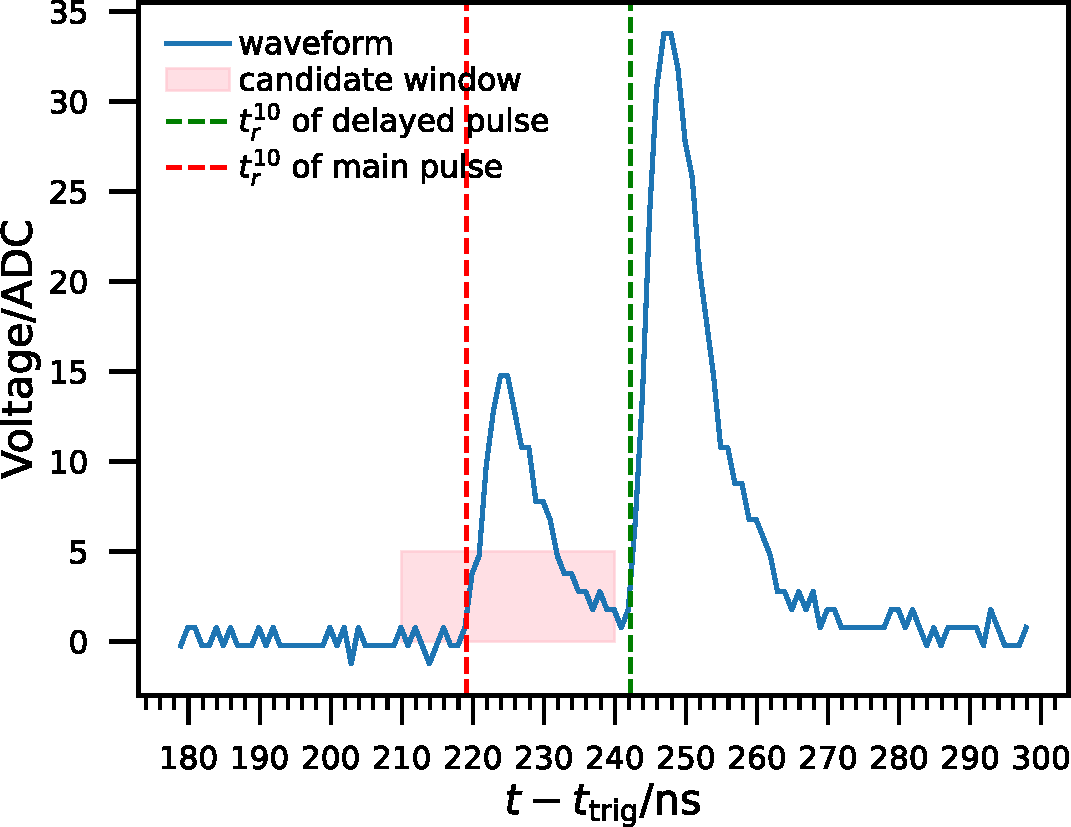
\includegraphics[width=\textwidth]{figures/method/triggerDoublePulse.pdf}
        \caption{}%PM
        \label{fig:triggerTT2pulse}
    \end{subfigure}
    \caption{(a) The drift schema of electrons between cathode and MCP. (b) Double pulses example. The first pulse fall in the candidate window.}
\end{figure}

The transit time (TT) of a PE is mainly composed of the drift time and multiplication time. The TTS is the spread of TT, which represents the resolution of timing. The transit time cannot be measured directly, while the trigger time of the laser and the time of pulse can be measured. A relative transit time $\mathrm{TT}_r$ is defined as the time difference between trigger time $t_{\mathrm{trig}}$ and $t_r^{10}$. The $\mathrm{TT}_r$ distribution of the MCP-PMTs contain two slow-falling edges on both sides of the peak as shown in Fig.~\ref{fig:triggerTTSLog} and Fig.~\ref{fig:triggerTTS}. The tail before the peak of TT distribution is due to the large kinetic energy of the photoelectron, which leads to a shorter TT. The tail on the other side is consisted of secondary electrons with a longer drift time.

To describe the delayed pulse after the main peak, main pulses are searched in the interval $[\mu_{t0}-5\,\mathrm{ns},\mu_{t0}+5\,\mathrm{ns}]$, while delayed pulses are searched in the interval $[\mu_{t0}+20\,\mathrm{ns},\mu_{t0}+80\,\mathrm{ns}]$. The blue histogram in Fig.~\ref{fig:triggerTTlatepulse} is the distribution of delayed pulses and the filled blue histogram is the distribution of delayed pulses with the existence of main pulses. The sharp difference between them at about \SI{40}{ns} after the main peak, twice times drift time of electrons from the cathode to the MCP, illustrates the delayed pulses lead by elastic scattering electrons cannot appear with the main pulse at the same time.

\begin{figure}[!htbp]
    \centering
    \begin{subfigure}[t]{\SF\textwidth}
        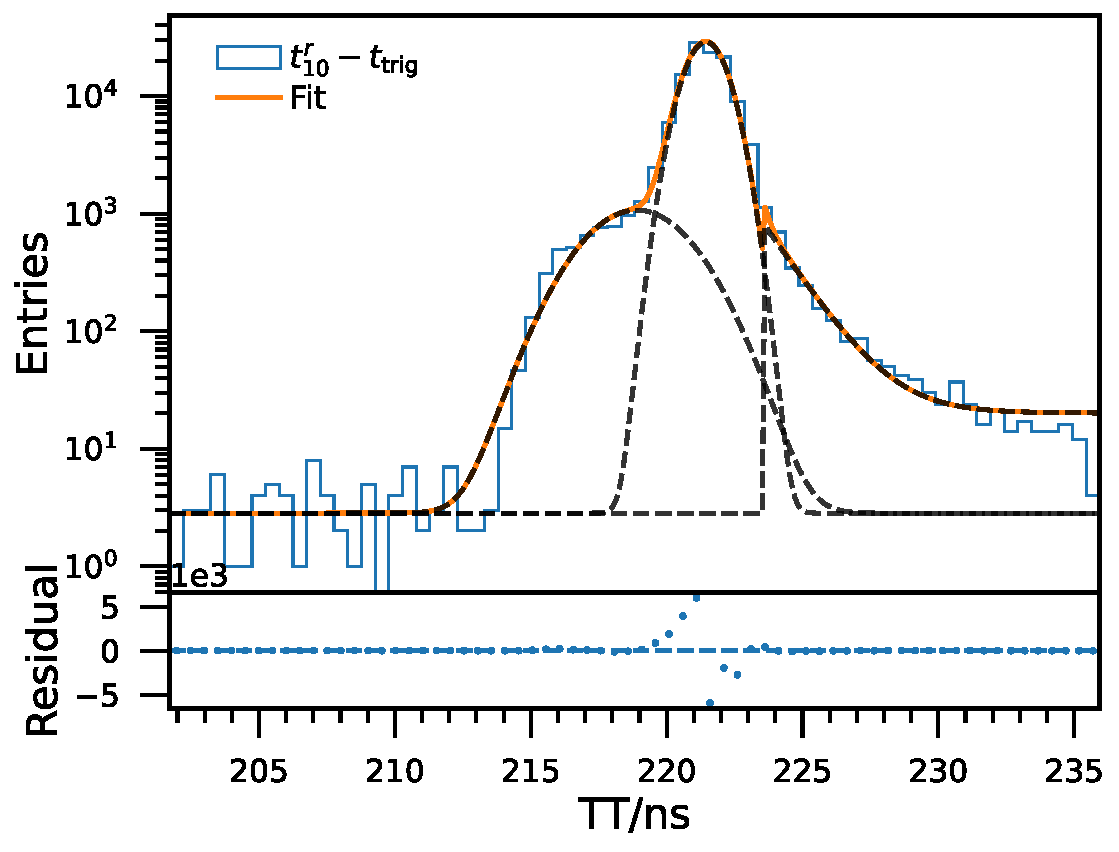
\includegraphics[width=\textwidth]{figures/method/triggerTTSLog.pdf}
        \caption{}%PM
        \label{fig:triggerTTSLog}
    \end{subfigure}
    \begin{subfigure}[t]{\SF\textwidth}
        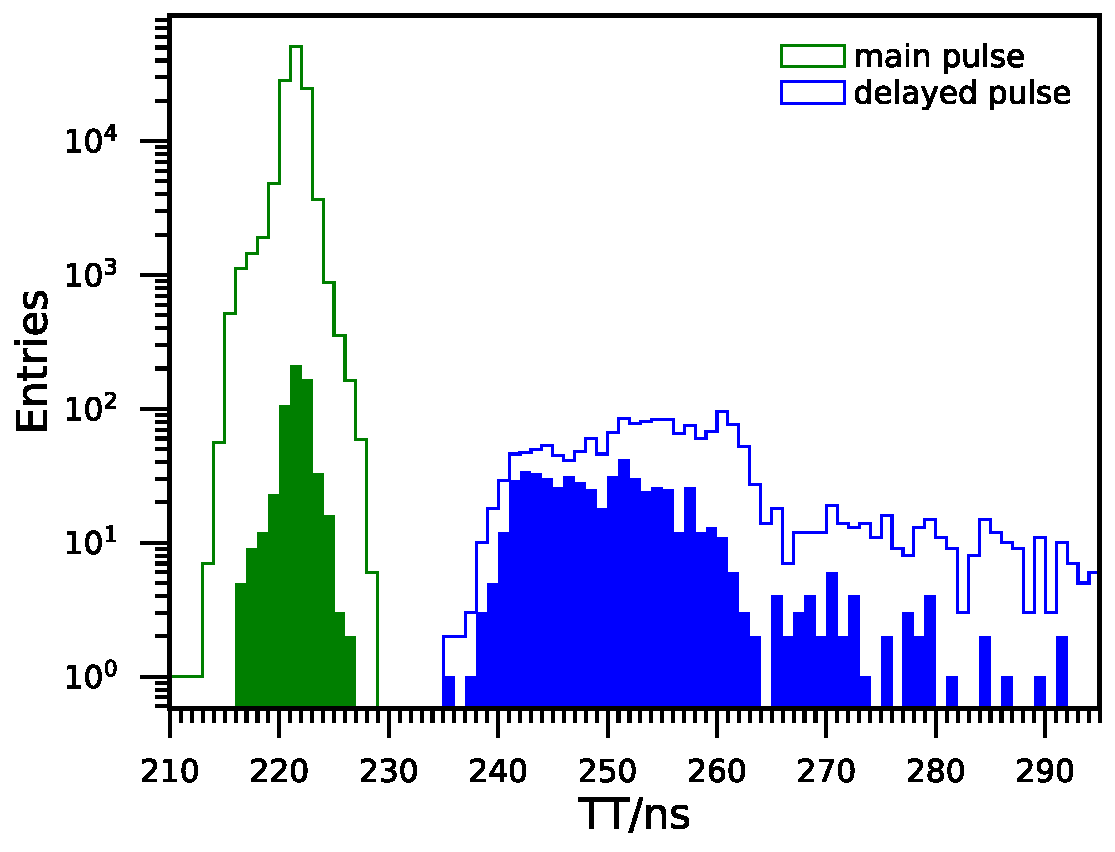
\includegraphics[width=\textwidth]{figures/method/triggerDelayedPulse.pdf}
        \caption{}%PM
        \label{fig:triggerTTlatepulse}
    \end{subfigure}
    \caption{(a) The distribution of TT with y-axis in logarithm sacle. The black dash line are 3 main components with a dark noise pedestal. (b) The green and blue histogram are respectively the main pulses distribution and delayed pulses distribution. The filled histogram are waveforms containing main pulses and delayed pulses at the same time.}
\end{figure}

The main peak and the tail before the main peak are modeled with Gaussian function $N_tG(\mu_{\mathrm{TT}},\sigma_{\mathrm{TT}}^2)$ and $N_KG(\mu_K,\sigma_K^2)$. Considering the distribution of kinetic energy of secondary electrons \cite{Furman,SecondElectron} and observed data, a phenomenological unphysical function $b_S+N_Se^{-\frac{t}{\tau_S}}$ is used to model the delayed pulse. Besides, to avoid the influence of unphysical function on $G(\mu_{\mathrm{TT}},\sigma_{\mathrm{TT}}^2)$, the function is translated to $\mu_{\mathrm{TT}}+2\sigma_{\mathrm{TT}}$.  As shown in Fig.~\ref{fig:triggerTTSLog} and Fig.~\ref{fig:triggerTTS}, the histogram of $\mathrm{TT}_r$ with \SI{0.5}{ns} bin width is binned fitted using following equation
\begin{equation}
    B+N_tG(\mu_{\mathrm{TT}},\sigma_{\mathrm{TT}}^2)+N_KG(\mu_K,\sigma_K^2)+H(\mu_{\mathrm{TT}}+2\sigma_{\mathrm{TT}})\left(b_S+N_Se^{-\frac{t-(\mu_{\mathrm{TT}}+2\sigma_{\mathrm{TT}})}{\tau_S}}\right)
\end{equation}
in which $H$ is the heaviside function to limit the unphysical exponential function, $B$ is the dark noise pedestal. TTS is defined as FWHM $2\sqrt{2\ln(2)}\sigma_{\mathrm{TT}}$ \cite{HAMAMATSUManual}. Fig.~\ref{fig:triggerTTS2d} also shows the long tail in charge distribution.

\begin{figure}[!htbp]
    \centering
    \begin{subfigure}[t]{\SF\textwidth}
        \includegraphics[width=\textwidth]{figures/method/triggerTTS.pdf}
        \caption{}%PM
        \label{fig:triggerTTS}
    \end{subfigure}
    \begin{subfigure}[t]{\SF\textwidth}
        \includegraphics[width=\textwidth]{figures/method/triggerTTS2d.pdf}
        \caption{}%PM
        \label{fig:triggerTTS2d}
    \end{subfigure}
    \caption{(a) The distribution of TT with y-axis in linear sacle. (b) The 2d distribution of TT and equivalent charge. The colorbar is in logarithm scale.}
\end{figure}

\subsection{Single electron response (SER)}
\begin{figure}
    \centering
    \includegraphics[width=\MF\textwidth]{figures/method/triggerSER.pdf}
    \caption{A fitting result of a pulse.}
    \label{fig:triggerser}
\end{figure}
To get a smooth single electron response (SER), the pulses are selected by dedicated cuts: the amplitude and charge of pulses should fulfill the criteria in sec.~\ref{sec:noisepeak}; the FWHM of candidate pulses should exceed \SI{2}{ns} and less than \SI{15}{ns} to avoid the noise and very large pulses; a charge filter $[0.5C_1, 1000\mathrm{ADC\cdot ns}]$ is used to remove the influence of fluctuation and outliers.

A gaussian function convoluted with an exponential function Equ~\eqref{equ:ser} is used to fit the SER which is shown in Fig.~\ref{fig:triggerser}.

\begin{equation}
    \label{equ:ser}
    \mathrm{Gaus}(0,\sigma_{\mathrm{ser}}^2)\otimes\theta(t-\mu_{\mathrm{ser}})\frac{1}{\tau_{\mathrm{ser}}}e^{-\frac{t-\mu_{\mathrm{ser}}}{\tau_{\mathrm{ser}}}}
\end{equation}
in which $\theta(t)$ is the unit step function, $\mu_{\mathrm{ser}}$ is the time offset of pulse, $\sigma_{\mathrm{ser}}$ and $\tau_{\mathrm{ser}}$ model the shape feature of SER. The results of $\tau_{\mathrm{ser}}$ and $\sigma_{\mathrm{ser}}$ of 9 MCP-PMTs are shown in Fig.~\ref{fig:sigmaCompare}.
\begin{figure}[!htbp]
    \centering
    \includegraphics[width=\MF\textwidth]{figures/result/tausigma.pdf}
    \caption{$\tau$ versus $\sigma$ of 9 MCP-PMTs.}
    \label{fig:sigmaCompare}
\end{figure}


\subsection{Pre-pulse and after-pulse}
\label{sec:afterpulse}
\begin{figure}
    \centering
    \includegraphics[width=\LF\textwidth]{figures/method/triggerAfterpulseSchema.pdf}
    \caption{Schema for searching pre-pulses and after-pulses. Green and red vertical dash lines are respectively the rising edge of trigger waveform and 10\% of rising edge of main pulse. The dark region and orange region are respectively the interval for searching after-pulses and pre-pulses.}
    \label{fig:afterpulseSchema}
\end{figure}

The generation of pre-pulses is due to photons hitting on the MCP or the first dynode directly rather than the photocathode \cite{JUNOMassTesting}. The amplitudes of pre-pulses are smaller than that of normal signals and pre-pulses appear before the main pulse about tens of nanoseconds \cite{JUNOMassTesting}. The after-pulse is generated due to the ionization of gaseous impurities between the cathode and first dynode or MCP when photoelectrons go through \cite{Coates_1973}. These ions hit back on the photocathode and generate electrons. \ce{H^+}, \ce{He^+}, \ce{O^+} are the major ions contributing to after-pulse and the relation between time and ions (\ce{^Z_MX}) is $\sqrt{\frac{M}{Z}}$, in which $M$ and $Z$ are the mass and charge of ions \cite{Coates_1973,XENON1TTesting}. Considering electric field and $\frac{M}{Z}$ of ions, the travel time is in the scale of \si{us}. The after-pulses are searched from \SI{200}{ns} after the main pulse and pre-pulses are searched from \SI{10}{ns} before the main pulse. The peak position $t_p$ and equivalent charge $C_{\mathrm{equ}}$ of the after-pulse and pre-pulse are calculated in the $[-10,75]$ ns window relative to the peak position as shown violet area in Fig.~\ref{fig:afterpulseSchema}.

\begin{figure}[!htbp]
    \centering
    \begin{subfigure}[t]{\LF\textwidth}
        \includegraphics[width=\textwidth]{figures/method/triggerAfterpulse1d.pdf}
        \caption{}%PM
        \label{fig:afterpulse1d}
    \end{subfigure}
    \begin{subfigure}[t]{\LF\textwidth}
        \includegraphics[width=\textwidth]{figures/method/triggerAfterpulse2d.pdf}
        \caption{}
        \label{fig:afterpulse2d}
    \end{subfigure}
    \caption{(a) Time distribution of pre-pulses and after-pulses. The orange and blue histograms are respectively ditributions of pre-pulses and after-pulses. The green line is the fit result for the distribution of after-pulses. The blank area around the \SI{0}{ns} is the main pulses which are not shown in this figure. (b) Charge vs time distribution of pre-pulses and after-pulses.}
\end{figure}
% waveform analysis

The relative t is defined as the difference between $t_p$ of pre/after-pulse and $t_r^{10}$ of main pulse. The distribution of relative t is shown in Fig.~\ref{fig:afterpulse1d}. The histogram with binwidth $T_{\mathrm{bin}}=10\mathrm{ns}$ indicates 4 typical after-pulse peaks in time around \SI{300}{ns}, \SI{550}{ns}, \SI{1200}{ns} and \SI{1700}{ns}, of which ratio is about $1:\sqrt{3}:\sqrt{16}:\sqrt{32}$. Considering the different mass of ions, these peaks may originate from \ce{H^+}, \ce{He^{+}} or other unknown ions, \ce{O^+} or \ce{CH_4^+}, and \ce{O_2^+} or other unknown ions. XENON1T and XMass gave similar assumptions for the first two peaks of after-pulse distribution \cite{XENON1TTesting, Abe_2020}. Other similar works done by JUNO and KM3NeT claimed the first peak is \ce{H_2^{+}} for the \SI{20}{inch} PMT \cite{Zhao:2022gks,KM3NetTesting}. Double Chooz proposed an unclear assumption for those peaks for R7081 PMT \cite{Haser_2013}.

The time distribution and ratio of different peaks in after-pulse distribution are parameterized using 4 gaussian functions (Equ.~\eqref{equ:afterpulse}) to model the four peaks after substracting dark noise rate $N_{\mathrm{DCR}}$. $N_{\mathrm{DCR}}$ is estimated as $N_{\mathrm{trig}}\cdot \mathrm{DCR}\cdot T_{\mathrm{bin}}$, in which $N_{\mathrm{trig}}$ is the number of triggered waveforms and DCR is calculated as sec.~\ref{sec:dcr}. The fit equation is as follows

\begin{equation}
    \label{equ:afterpulse}
    \sum_{i=1}^{4}{A_iG(t_i,\sigma_i^2)}
\end{equation}
in which $A_i$, $t_i$, and $\sigma_i$ are the ratio factor, time, width of each peak of after-pulse. The fit results are shown in Fig.~\ref{fig:afterpulsePeak} and the ratios of the 4 peaks vary greatly for different MCP-PMTs. Besides, there exist some areas that cannot be well modeled with Equ.\eqref{equ:afterpulse}, for example, the pedestal between the first and second peaks of after-pulse distribution. The mean and standard deviation of fit results are summarized in Table.~\ref{tab:afterpulse}. Due to the influence of after-pulses around the second peak, the standard deviation of $\sigma_2$ is very large.
\begin{figure}[!htbp]
    \centering
    \includegraphics[width=\MF\textwidth]{figures/result/afterpulse.pdf}
    \caption{Time and relative ratio of peaks of after-pulse ratios of 9 MCP-PMTs. 4 peak ratios are plotted along the time for each PMT.}
    \label{fig:afterpulsePeak}
\end{figure}

% Fig.\ref{fig:afterpulse2d} indicates that the after pulse contains some very large signal in the specific peaks, which is different from the distribution of single PE.
\begin{table}
    \centering
    \caption{Parameters of after-pulse of 9 MCP-PMTs}
    \label{tab:afterpulse}
    \begin{tabular}{c|c|c|c|c}
        \hline
        &1st peak&2nd peak&3rd peak&4th peak\\
        $t_i$/ns&304$\pm$6&563$\pm$21&1196$\pm$39&1722$\pm$24\\
        $A_i/A_1$&1&0.73$\pm$0.26&1.23$\pm$0.47&2.2$\pm$1.1\\
        $\sigma_i$/ns&8.8$\pm$2.1&81$\pm$28&61$\pm$24&69$\pm$26\\
        \hline
    \end{tabular}
\end{table}

The ratio of pre-pulses $R_{\mathrm{pre}}$ is calculated in time interval [-150,-10]\,ns and after-pulses $R_{\mathrm{after}}$ is calculated in time interval [200,9800]\,ns as following equations

\begin{align}
    R_{\mathrm{pre}} = \frac{N_{\mathrm{pre}}}{N_\mathrm{trig}} - \mathrm{DCR}\cdot T_{\mathrm{pre}}\\
    R_{\mathrm{after}} = \frac{N_{\mathrm{after}}}{N_\mathrm{trig}} - \mathrm{DCR}\cdot T_{\mathrm{after}}
\end{align}
in which $T_{\mathrm{pre}}=140$\,ns, $T_{\mathrm{after}}=9600$\,ns, $N_{\mathrm{pre}}$ and $N_{\mathrm{after}}$ are the number of pre-pulses and after-pulses, DCR is calculated as sec.~\ref{sec:dcr}. Due to the ratio of pre-pulse is too small, some measured values are smaller than zero after deducting DCR as shown in Fig.~\ref{fig:prepulseCompare}.

\begin{figure}[!htbp]
    \centering
    \includegraphics[width=\MF\textwidth]{figures/result/preafterpulse.pdf}
    \caption{pre-pulse ratio versus after-pulse ratio.}
    \label{fig:prepulseCompare}
\end{figure}

\subsection{Dark count rate (DCR)}
\label{sec:dcr}
The dark noise mainly comes from the spontaneous thermionic electrons emitted from the photocathode \cite{KM3NetTesting}, which generates a pulse signal similar to a photoelectron. The DCR equals the following equation

\begin{equation}
    \mathrm{DCR/kHz} = \frac{N_{\mathrm{noise}}}{N_{\mathrm{trig}}}\frac{1}{T_{\mathrm{DCR}}/\mathrm{ns}}\times 10^{6}
\end{equation}
in which $N_{\mathrm{noise}}$ is the noise number in the interval of $[-200,-150]$\ ns relative to main pulse, and $T_{\mathrm{DCR}}$ is \SI{50}{ns}. The DCRs of MCP-PMTs are illustrated in Fig.~\ref{fig:DCRCompare}.

\begin{figure}[!htbp]
    \centering
    \includegraphics[width=\MF\textwidth]{figures/result/DCRPDE.pdf}
    \caption{Relative PDE versus DCR of 9 MCP-PMTs.}
    \label{fig:DCRCompare}
\end{figure}

\subsection{Relative photon detection efficiency (PDE)}
The DCR is omitted in the PDE calculation due to the small ratio of dark noise. To measure PDE, the intensity of light and light allocation ratio of each channel of the laser splitter need to be calibrated. For example, JUNO fixed one reference PMT to calibrate the light intensity and other reference PMTs are circulated through all channels to calibrate the light allocation ratio \cite{Wonsak_2021}. A new method is designed to reduce the number of reference PMT to 1 PMT and could combine all test runs to do the calibration in this work.

Note $n,j,k$ ($n=0,...,N-1, j=0,...,J-1, k=0,...,K-1$) is the indicator of the test runs, the channels of the splitter and the PMTs. The intensity of light is $I_n$, light allocation ratio is $\alpha_j$ and PDE is $\eta_k$. Assume $\alpha_j$s are stable among different test runs. $N_t$ is the total number of waveforms. The photon numbers in each waveform obey Poisson distribution $\pi(p_{njk})$, in which $p_{njk}=I_n\alpha_j\eta_k$. The trigger rate of nth run, kth PMT in jth channel is

\begin{equation}
    \label{equ:pderate}
    R_{njk}=1-e^{-p_{njk}}
\end{equation}
For convenience, 0th PMT is the only one reference PMT. Note $\alpha_j^0=\frac{\alpha_j}{\alpha_0}$, $\eta_k^0=\frac{\eta_k}{\eta_0}$, $I_n^0=I_n\alpha_0\eta_0$, $i\equiv njk$. Therefore, $p_{njk}$ can be transfer to Equ~\eqref{equ:pdelograte}

\begin{equation}
    \label{equ:pdelograte}
    \mathrm{log}(p_{i})=\mathrm{log}(I_0\alpha_0\eta_0)+\mathrm{log}(I_n^0)+\mathrm{log}(\alpha_j^0)+\mathrm{log}(\eta_k^0)
\end{equation}
The relationship between $R_{i}$ and parameters is

\begin{equation}
    \label{equ:linkfunction}
    R_{i}=1-e^{-e^{\mathrm{log}(I_0\alpha_0\eta_0)+\mathrm{log}(I_n^0)+\mathrm{log}(\alpha_j^0)+\mathrm{log}(\eta_k^0)}}
\end{equation}
The trigger number $N_{{\mathrm{trig}_{i}}}$ of kth PMT in nth run with jth splitter obey Binomial distribution $B(R_{i},N_{t_{i}})$, in which $N_{t_{i}}$ is total number of waveforms. To fit the parameters, a likelihood is constructed as follows

\begin{equation}
    \label{equ:likelihood}
    \mathcal{L}=\prod_{i}{R_{i}^{N_{\mathrm{trig}_{i}}}(1-R_{i})^{N_{t_{i}}-N_{\mathrm{trig}_{i}}}}
\end{equation}

The relationship in Equ.~\eqref{equ:linkfunction} matches the general linear model (GLM) of Binomial exponential family distribution with Cloglog link function \cite{glm}. The GLM is used to maximize the likelihood in Equ.~\eqref{equ:likelihood} and calculate the best value of $\mathrm{log}(\eta_k^0)$ and $\mathrm{log}(\alpha_k^0)$, which is used to calibrate relative PDEs and splitter ratios. The results of PDE are shown in Fig.~\ref{fig:DCRCompare}. The mean of relative PDE is about $1.71$, which is obviously higher than the reference PMT.

The mean and standard deviation of parameters of 9 MCP-PMTs are summarized in Table~\ref{tab:summary}.
\begin{table}
    \centering
    \caption{charge and time characteristic of 9 MCP-PMTs}
    \label{tab:summary}
    \begin{tabular}{c| r @{$\pm$} l}
        Parameter&\multicolumn{2}{c}{$\mu\pm\sigma$}\\
        \hline
        $G_1$/1E7&1.19&0.07\\
        $G$/1E7&2.1&0.2\\
        $\mathrm{Res}_1$&0.25&0.02\\
        Res&0.69&0.03\\
        TTS/ns&1.68&0.09\\
        DCR/kHz&4.5&1.3\\
        $\tau_{\mathrm{ser}}$/ns&7.2&1.0\\
        $\sigma_{\mathrm{ser}}$/ns&1.62&0.06\\
        relative PDE&1.71&0.06\\
        $R_{\mathrm{pre}}$&$8\times10^{-5}$&$1.6\times10^{-4}$\\
        $R_{\mathrm{after}}$&0.013&0.004\\
        \hline
    \end{tabular}
\end{table}
